%!TEX root = ../agi_mfwis415af4l.tex
\section{Dokumentation der Software}
\label{concept}

\subsection{Dokumentation der Paketstruktur des Android-Projektes}

\subsection{Dokumentation der Activities}\\


\subsubsection{Activity 1}
\setcounter{tocdepth}{4} 
\setcounter{secnumdepth}{4}
\paragraph{Aufgabe und Funktion}\\
Die Main-Activity umfasst die Startseite der Applikation. Im Header sichtbar ist ein Fortschrittsbalken, der die konsumierten Kalorien mit dem Tagesbedarf an Kalorien gegenüberstellt. Diese Auskunft ist nicht nur visuell, sondern auch textuell hinterlegt mit exakten Werten. In der Fußleiste der Activity findet sich eine Navigationsleiste wieder. In dieser sind vier Knöpfe zu sehen. Das linke Icon zeigt einen Kalender, der Sie beim Klicken in die Kalender-Übersicht bringt. Der Knopf rechts daneben ist betitelt mit „Lebensmittel“. Bei Klick darauf gelangt man in die Lebensmittelübersicht. Der nächste Knopf mit dem Namen „Menüs“ lässt Sie in die Übersicht der Menüs gelangen. Der letzte Knopf der Navigationsleiste zeigt ein Profilicon. Bei Klick auf das Icon gelangen Sie in Ihre persönliche Profilübersicht, bei der Sie die Daten bezüglich ihres Gewichtes, der Größe und den Tagesbedarf an Kalorien ändern können.
In der Mitte befinden sich die einzelnen Tageszeiten „Frühstück“, „Mittagessen“, „Abendessen“ und „Snacks“, bei denen man bei Klick auf das rote Plus eine Mahlzeit zur jeweiligen Tageszeit hinzufügen kann. Hierbei wird man auf ein neues Fenster geleitet in der man das Lebensmittel oder ein Menü, die dazugehörige Menge und die Einheit auswählen kann. Die Kalorien werden ausgerechnet und sind nicht veränderbar.

\paragraph{Layout, Screenshot(s)}\\
\paragraph{Use-Case}$~~$\\
\newline
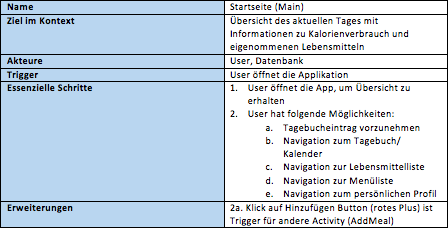
\includegraphics[scale=1]{img/usecasemain}\\
\paragraph{Datenverwaltung innerhalb der Activity}\\
Anzeige: Die gewünschten Parameter werden aus dem entsprechendem Eintrag in der Kalorientagebuchtabelle mit Hilfe der Tageszeit und dem Datum in dem Layout angezeigt.

\paragraph{Datenschnittstellen zu anderen Activity}\\
Beim Hinzufügen eines Tagebucheintrags wird die Tageszeit und das Datum als Parameter mitgegeben. Der Tageshöchstwert wird aus der Datenbank-Profiltabelle entnommen. 

\paragraph{Dokumentation des Quelltextes der Activity}\\

\subsubsection{Activity 2}

\paragraph{Aufgabe und Funktion}\\
Die Activity „Kalender“ ist horizontal in zwei Abschnitte geteilt. In dem oberen Teil befindet sich ein Kalender den man durch einfaches Wischen und Klicken bedienen kann. Bei der Ansicht wird der aktuelle Monat angezeigt.
In dem unteren Teil der Activity befindet sich die Übersicht aus der Startseite über die Tageszeiten mit der Möglichkeit Mahlzeiten hinzuzufügen. Hier kann der Benutzer entweder zu dem aktuellen Tag weiter Lebensmittel oder Menüs hinzufügen oder zu einem vergangenen Tag eine Mahlzeit hinzufügen. Außerdem ist er in der Lage auf eine bestimmte Mahlzeit an einem bestimmten Tag zu klicken und somit in ein neues Fenster navigieren, in dem er die Mahlzeit nach Belieben verändern kann. 

\paragraph{Layout, Screenshot(s)}\\
\paragraph{Use-Case}$~~$\\
\newline
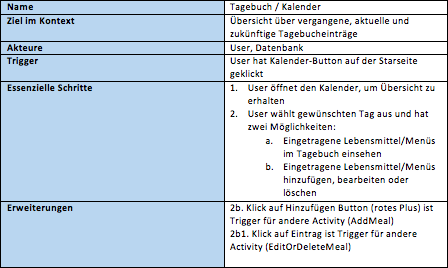
\includegraphics[scale=1]{img/usecasecalendar}\\
\paragraph{Datenverwaltung innerhalb der Activity}\\
Anzeige: Die gewünschten Parameter werden aus dem entsprechendem Eintrag in der Kalorientagebuchtabelle mit Hilfe der Tageszeit und dem Datum in dem Layout angezeigt.

\paragraph{Datenschnittstellen zu anderen Activity}\\
Beim Hinzufügen eines Tagebuchseintrags wir die spezifische Tageszeit und das Datum mitgegeben.

\paragraph{Dokumentation des Quelltextes der Activity}\\

\subsubsection{Activity 3}

\paragraph{Aufgabe und Funktion}\\
Die Activity bietet eine Übersicht über die, vom User angelegten, Lebensmitteln in der Datenbank. Außerdem kann der Nutzer per Klick auf „Lebensmittel hinzufügen“ in ein Fenster weitergeleitet werden, in dem er neue Lebensmittel hinzufügen kann. Des Weiteren ermöglicht der Klick auf ein Lebensmittel die Bearbeitung oder Löschung des gewählten Lebensmittels.

\paragraph{Layout, Screenshot(s)}\\
\paragraph{Use-Case}$~~$\\
\newline
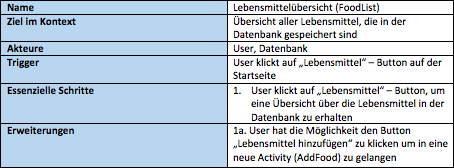
\includegraphics[scale=1]{img/usecasefoodlist}\\
\paragraph{Datenverwaltung innerhalb der Activity}\\
Anzeige: Die jeweiligen Parameter werden aus dem entsprechenden Eintrag der Tabelle der Lebensmittel in das Layout geladen. 

\paragraph{Datenschnittstellen zu anderen Activity}\\
Der Hinzufügen-Button leitet lediglich auf die entsprechende Activity weiter.

\paragraph{Dokumentation des Quelltextes der Activity}\\

\subsubsection{Activity 4}

\paragraph{Aufgabe und Funktion}\\
In der Activity „Lebensmittel hinzufügen“ kann der Benutzer ein neues Lebensmittel in seiner Applikation hinzufügen. Dieses Lebensmittel kann er im Anschluss als Mahlzeit in seinem Tagebuch verwenden oder in ein Menü seiner Wahl hinzufügen.
Folgende Informationen zu dem Lebensmittel müssen ausgefüllt werden um ein Lebensmittel erfolgreich zu der Datenbank hinzufügen zu können: 
\begin{itemize}
\item Name
\item Beschreibung
\item Anzahl + Einheit
\item Kalorien
\end{itemize}

Bei erfolgreichen Hinzufügen wird das Lebensmittel nun in der Lebensmittelübersicht angezeigt.

\paragraph{Layout, Screenshot(s)}\\
\paragraph{Use-Case}$~~$\\
\newline
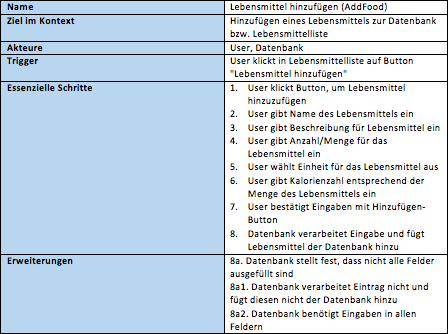
\includegraphics[scale=1]{img/usecaseaddfood}\\
\paragraph{Datenverwaltung innerhalb der Activity}\\
Anzeige: Die Einheiten werden aus der Tabelle der Einheiten geladen und im Spinner aufgelistet. 
Hinzufügen: Ein neuer Eintrag wird in der Tabelle der Lebensmittel hinzugefügt, indem die Parameter vom Layout weitergegeben werden. 

\paragraph{Datenschnittstellen zu anderen Activity}\\
Schnittstelle zur Einheiten und Entsprechungen Activities vorhanden, um Parameter zu laden und anzuzeigen. 

\paragraph{Dokumentation des Quelltextes der Activity}\\

\subsubsection{Activity 5}

\paragraph{Aufgabe und Funktion}\\
In der EditOrDeleteFood-Activity hat der User die Möglichkeit, seine Einträge aus der Lebensmittelliste zu bearbeiten oder komplett zu löschen. So können alle zuvor eingetragenen Parameter wie Name, Beschreibung, Anzahl/Menge geändert werden. Dabei bleibt die zuvor eingetragene Einheit jedoch erhalten und kann nicht editiert werden. Zusätzlich kann der User anschließend die Kalorienzahl entsprechend der neuen Parameter eintragen. Zum Speichern des geänderten Lebensmittels steht hierfür der Speichern-Button zur Verfügung. Soll das Lebensmittel jedoch dauerhaft aus der Lebensmittelliste gelöscht werden, so genügt ein Klick auf den Löschen-Button. 

\paragraph{Layout, Screenshot(s)}\\
\paragraph{Use-Case}$~~$\\
\newline
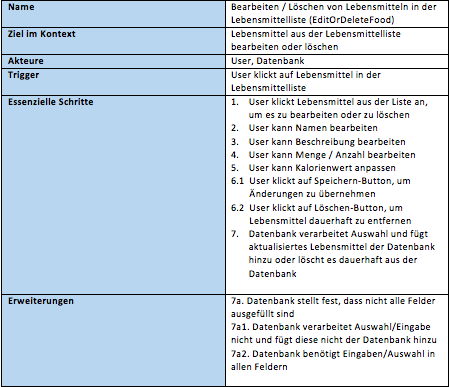
\includegraphics[scale=1]{img/usecaseeodfood}\\
\paragraph{Datenverwaltung innerhalb der Activity}\\
Anzeige: Die jeweiligen Parameter werden aus dem entsprechenden Eintrag der Tabelle der Lebensmittel und der Entsprechungen in das Layout geladen. 
Bearbeiten: Die Parameter werden angepasst, indem der aufgerufene Eintrag unverändert in der Datenbank mit einem sogenannten „IS-ACTIVE Flag" auf 0 beziehungsweise „false“ gesetzt wird. Dadurch werden bereits eingetragene Lebensmittel im Kalorientagebuch nicht verändert. Zusätzlich dazu wird ein komplett neuer Eintrag erstellt, der mit den geänderten Parametern bestückt ist. In der Lebensmittelliste wird nun der neue Eintrag angezeigt und der alte Eintrag ausgeblendet. 
Löschen: Das Lebensmittel bleibt passiv in der Datenbank gespeichert (Flag „IS-ACTIVE“ wird in der Tabelle auf 0 bzw. "false" gesetzt), um alte Einträge mit dem Lebensmittel nicht ebenfalls aus dem Tagebuch zu löschen. Das gelöschte Lebensmittel wird jedoch nicht mehr in der Lebensmittelliste angezeigt.

\paragraph{Datenschnittstellen zu anderen Activity}\\
Schnittstelle zur Lebensmittelliste (Activity Food List)

\paragraph{Dokumentation des Quelltextes der Activity}\\

\subsubsection{Activity 6}

\paragraph{Aufgabe und Funktion}\\
In der Activity „Menü-Übersicht“ werden alle erstellten Menüs in tabellarischer Form angezeigt. Der Nutzer kann auf den Button „Menü hinzufügen“ klicken um ein neues von ihm erstelltes Menü zu der Datenbank hinzuzufügen. Außerdem kann der User auf ein Menü klicken um es dann zu bearbeiten oder zu löschen.

\paragraph{Layout, Screenshot(s)}\\
\paragraph{Use-Case}$~~$\\
\newline
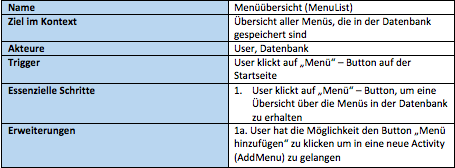
\includegraphics[scale=1]{img/usecasemenulist}\\
\paragraph{Datenverwaltung innerhalb der Activity}\\
Anzeige: Die jeweiligen Parameter werden aus dem entsprechenden Eintrag der Tabelle der Menüs in das Layout geladen. 

\paragraph{Datenschnittstellen zu anderen Activity}\\
Der Menü Hinzufügen Button leitet lediglich zur entsprechenden Activity weiter.

\paragraph{Dokumentation des Quelltextes der Activity}\\

\subsubsection{Activity 7}

\paragraph{Aufgabe und Funktion}\\
In der Activity „Menü hinzufügen“ kann mein Menü hinzufügen. Ein Menü besteht aus mindestens einem Lebensmittel. Das Menü muss einen Namen und eine Beschreibung haben um dies zu der Datenbank hinzufügen zu können. Die Lebensmittel können mit einer Checkbox ähnlichen ListView ausgewählt werden. Mit Hilfe des Buttons „Hinzufügen“ wird das Menü zu der Datenbank hinzugefügt.

\paragraph{Layout, Screenshot(s)}\\
\paragraph{Use-Case}$~~$\\
\newline
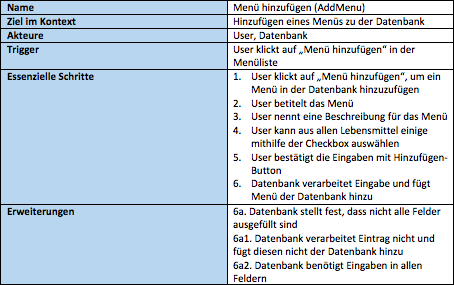
\includegraphics[scale=1]{img/usecaseaddmenu}\\
\paragraph{Datenverwaltung innerhalb der Activity}\\
Anzeige: Die jeweiligen Parameter werden aus dem entsprechenden Eintrag der Tabelle der Lebensmittel in das Layout geladen. 
Hinzufügen: Die eingegebenen Parameter werden in einem neuen Eintrag der Menütabelle der Datenbank gespeichert. Die korrespondieren Lebensmittel eines Menüs werden in der Zuweisungstabelle von Menü-IDs und Lebensmittel-IDs gespeichert. 

\paragraph{Datenschnittstellen zu anderen Activity}\\
Die Lebensmittel-Übersicht bedient sich der Lebensmittel Activity. 

\paragraph{Dokumentation des Quelltextes der Activity}\\

\subsubsection{Activity 8}

\paragraph{Aufgabe und Funktion}\\
In der EditOrDeleteMenu-Activity hat der User die Möglichkeit seine zuvor eingetragenen Menüs aus der Menü-Liste zu bearbeiten oder zu löschen. So können neben dem Namen und der Beschreibung des Menüs auch die Lebensmittel angepasst werden. Hierfür steht dem User eine Checkbox zur Verfügung, über welche er die Lebensmittel einfach aus- oder abwählen kann. Mithilfe des Speichern-Buttons werden alle vorgenommenen Änderungen übernommen und in der Menü-Liste gespeichert. Soll das Menü jedoch dauerhaft aus der Menü-Liste entfernt werden, so genügt ein Klick auf den Löschen-Button.

\paragraph{Layout, Screenshot(s)}\\
\paragraph{Use-Case}$~~$\\
\newline
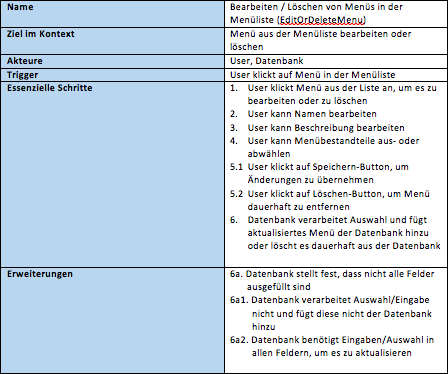
\includegraphics[scale=1]{img/usecaseeodmenu}\\
\paragraph{Datenverwaltung innerhalb der Activity}\\
Anzeige: Die Parameter werden aus dem entsprechendem Eintrag in der Tabelle der Menüs und der Menüs-Lebensmittel-Zuordnung geladen und im Layout angezeigt. 
Bearbeiten: Der aufgerufene Eintrag wird mit einem Flag auf inaktiv gesetzt und ein neuer Eintrag wird mit den entsprechenden Parametern erstellt. Die Tabelle Menüs und die Tabelle der Zuordnungen kriegen jeweils mindestens einen neuen Eintrag mit den entsprechenden IDS. 
Löschen: Das Menü bleibt passiv in der Datenbank gespeichert (Flag „IS-ACTIVE“ wird in der Tabelle auf 0 bzw. "false" gesetzt), um alte Einträge mit dem Menü nicht ebenfalls aus dem Tagebuch zu löschen. Das gelöschte Menü wird jedoch nicht mehr in der Menüliste angezeigt.

\paragraph{Datenschnittstellen zu anderen Activity}\\
Schnittstelle zur Menüliste (MenuList-Activity)

\paragraph{Dokumentation des Quelltextes der Activity}\\

\subsubsection{Activity 9}

\paragraph{Aufgabe und Funktion}\\
Das Profil des Benutzers wird von dem Benutzer selber ausgefüllt. Der Name, die Größe, das Gewicht, das Geburtsdatum und der Kalorientageshöchstwert werden hier festgelegt. Mit dem Button „Aktualisieren“ werden die „alten“ Daten mit den aktuellen Daten überschrieben. Der Knopf „Einheiten-Übersicht“ navigiert den User zu der Einheiten-Übersicht. Mithilfe des Button „Statistische Auswertung“ wird der Nutzer zu einem Fenster mit einer Übersicht seiner durchschnittlich aufgenommenen Kalorien in einem bestimmten Zeitraum geleitet.

\paragraph{Layout, Screenshot(s)}\\
\paragraph{Use-Case}$~~$\\
\newline
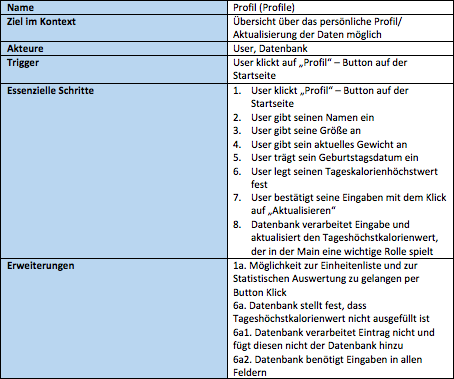
\includegraphics[scale=1]{img/usecaseprofile}\\
\paragraph{Datenverwaltung innerhalb der Activity}\\
Anzeige: Die jeweiligen Parameter werden aus dem entsprechenden Eintrag der Tabelle des Profils in das Layout geladen. 
Aktualisieren: Die Parameter werden aktualisiert, indem der Eintrag in der Profiltabelle der Datenbank gemäß den geänderten Werten angepasst wird.

\paragraph{Datenschnittstellen zu anderen Activity}\\
Die Main Activity greift auf den Tageshöchstwert des im Profil festgelegten Wertes zu.

\paragraph{Dokumentation des Quelltextes der Activity}\\

\subsubsection{Activity 10}

\paragraph{Aufgabe und Funktion}\\
In der Statistics-Activity hat der User die Möglichkeit, seine durchschnittlichen aufgenommenen Kalorien der letzten 7 Tage, 14 Tage und 30 Tage einzusehen. 

\paragraph{Layout, Screenshot(s)}\\
\paragraph{Use-Case}$~~$\\
\newline
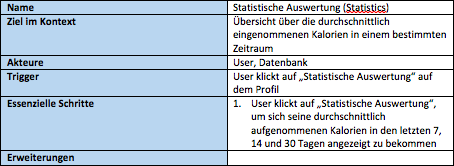
\includegraphics[scale=1]{img/usecasestatistics}\\
\paragraph{Datenverwaltung innerhalb der Activity}\\
Anzeige: Die Parameter werden aus dem entsprechendem Eintrag in der Kalorientagebuchtabelle geladen, jeweils spezifisch berechnet und anschließend im Layout angezeigt. 

\paragraph{Datenschnittstellen zu anderen Activity}\\
Schnittstelle zum Tagebuch (Calendar-Activity)

\paragraph{Dokumentation des Quelltextes der Activity}\\

\subsubsection{Activity 11}

\paragraph{Aufgabe und Funktion}\\
In dieser Activity sieht der Benutzer eine Übersicht über die verfügbaren Einheiten. Diese kann er mit dem Klick auf „Einheiten hinzufügen“ erweitern. Eine weitere Möglichkeit für den User liegt in dem Klicken auf eine Einheit, woraus sich ein neues Fenster zu Bearbeiten oder Löschen der Einheit.

\paragraph{Layout, Screenshot(s)}\\
\paragraph{Use-Case}$~~$\\
\newline
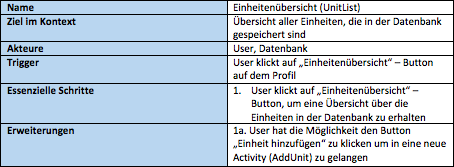
\includegraphics[scale=1]{img/usecaseunitlist}\\
\paragraph{Datenverwaltung innerhalb der Activity}\\
Anzeige: Die jeweiligen Parameter werden aus dem entsprechenden Eintrag der Tabelle der Einheiten in das Layout geladen. 

\paragraph{Datenschnittstellen zu anderen Activity}\\
Der Einheiten Hinzufügen Button leitet lediglich zur entsprechenden Activity weiter.

\paragraph{Dokumentation des Quelltextes der Activity}\\

\subsubsection{Activity 12}

\paragraph{Aufgabe und Funktion}\\
In dieser Activity hat der User die Möglichkeit eine neue Einheit zu der Datenbank hinzuzufügen. Für diese Aktion wird ein Name benötigt der die Einheit beschreibt. Mit dem Klick auf „Hinzufügen“ wird die Einheit der Datenbank hinzugefügt.

\paragraph{Layout, Screenshot(s)}\\
\paragraph{Use-Case}$~~$\\
\newline
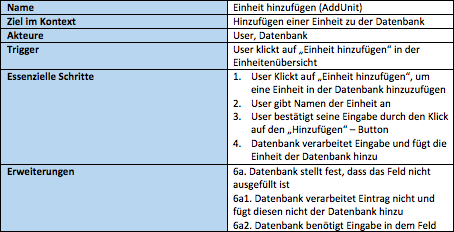
\includegraphics[scale=1]{img/usecaseaddunit}\\
\paragraph{Datenverwaltung innerhalb der Activity}\\
Hinzufügen: Die eingegebenen Parameter werden in einem neuen Eintrag der Einheitentabelle hinzugefügt.

\paragraph{Datenschnittstellen zu anderen Activity}\\
Die hinzugefügten Einheiten werden in der Lebensmittel Activity verwendet. 

\paragraph{Dokumentation des Quelltextes der Activity}\\

\subsubsection{Activity 13}

\paragraph{Aufgabe und Funktion}\\
In der EditOrDeleteUnit-Activity hat der User die Möglichkeit den Namen einer ausgewählten Einheit aus der Einheitenliste zu bearbeiten oder zu löschen. Über den Speichern-Button werden die Änderungen übernommen und in der Einheiten-Liste gespeichert. Soll die Einheit jedoch dauerhaft aus der Liste entfernt werden, so genügt ein Klick auf den Löschen-Button.

\paragraph{Layout, Screenshot(s)}\\
\paragraph{Use-Case}$~~$\\
\newline
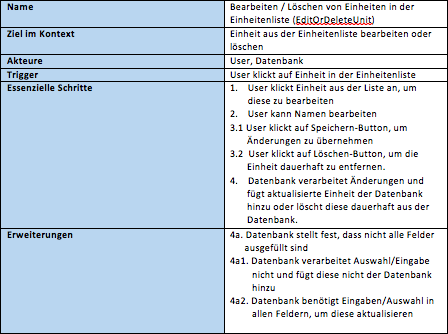
\includegraphics[scale=1]{img/usecaseeodunit}\\
\paragraph{Datenverwaltung innerhalb der Activity}\\
Anzeige: Die Parameter werden aus dem entsprechendem Eintrag in der Tabelle der Einheiten geladen und im Layout angezeigt. 
Bearbeiten: Die Änderungen werden übernommen und in der Datenbank gespeichert. 
Löschen: Die Einheit bleibt passiv in der Datenbank gespeichert (Flag „IS-ACTIVE“ wird in der Tabelle auf 0 beziehungsweise "false" gesetzt), um alte Einträge mit der Einheit nicht ebenfalls aus dem Tagebuch zu löschen.

\paragraph{Datenschnittstellen zu anderen Activity}\\
Schnittstelle zur Einheiten-Liste (Unit List-Activity)

\paragraph{Dokumentation des Quelltextes der Activity}\\

\subsubsection{Activity 14}

\paragraph{Aufgabe und Funktion}\\
In die Activity „Tagebucheintrag hinzufügen“ kommt der Benutzer durch das Klicken des roten Plus auf der Startseite oder im Kalender. Hier kann der Nutzer einen Eintrag hinzufügen zu dem aktuellen Tag, wenn er aus der Startseite kommt. Wenn der Nutzer in dem Kalender auf das Plus klickt, wird der ausgewählte Tag in die Activity übernommen. Der nächste Spinner, also eine Auswahl, stellt den Benutzer vor die Frage ob er die gewählte Tageszeit der Mahlzeit ändern möchte.
Die nächsten beiden Auswahleinheiten beziehen sich auf die Lebensmittel und Menüs. Hier kann der Benutzer per Spinner die gewünschte Mahlzeit auswählen. Die hinterlegte Einheit mit den jeweiligen Kalorien wird von der Applikation ausgefüllt und ist nicht mehr zu verändern. Die Menge wird auch von der App ausgefüllt, kann jedoch von dem Benutzer angepasst werden an die Mahlzeit, wie viel er gegessen hat. Die Kalorien passen sich dann je nach Menge der Mahlzeit an und werden angezeigt. Mithilfe des Buttons „Hinzufügen“ wird ein Tagebucheintrag in der Datenbank gespeichert.
\paragraph{Layout, Screenshot(s)}\\
\paragraph{Use-Case}$~~$\\
\newline
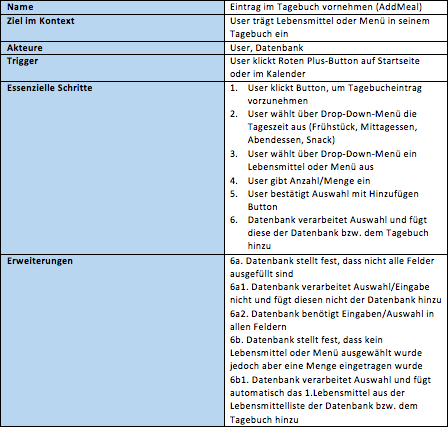
\includegraphics[scale=1]{img/usecaseaddmeal}\\
\paragraph{Datenverwaltung innerhalb der Activity}\\
Anzeige: Die jeweiligen Parameter werden aus dem entsprechenden Eintrag der Tabelle der Lebensmittel, Menüs und Entsprechungen in das Layout geladen. 
Hinzufügen: Die eingegebenen Parameter werden in einem neuen Eintrag der Kalorientagebuchtabelle gespeichert. 
\paragraph{Datenschnittstellen zu anderen Activity}\\
Das Datum und die Tageszeit werden von der vorherigen Activity gelesen und im Layout eingetragen.  
\paragraph{Dokumentation des Quelltextes der Activity}\\

\subsubsection{Activity 15}

\paragraph{Aufgabe und Funktion}\\
In der EditOrDeleteMeal-Activity hat der User die Möglichkeit, seine Einträge aus dem Tagebuch zu bearbeiten oder zu löschen. Soll der ausgewählte Eintrag komplett gelöscht werden, so steht hierfür der Löschen-Button zur Verfügung. Möchte der User jedoch lediglich seinen Eintrag bearbeiten, so können die Parameter Datum, Auswahl der Mahlzeit, Auswahl des Lebensmittel oder Menü sowie die Menge geändert werden. Über Änderungen am Parameter Datum, können die Einträge innerhalb des Tagebuches auf andere Tage im Kalender verschoben werden. Über ein Drop-Down Menü kann die Auswahl der Mahlzeit geändert werden, sodass Einträge beliebig zwischen Frühstück, Mittagessen, Abendessen oder Snacks verschoben werden können. Zudem dienen zwei weitere Drop-Down Menü zur Auswahl des Lebensmittels oder Menüs aus der Lebensmittelliste/Menüliste, sodass hier ein fälschlicherweise eingetragenes Lebensmittel oder Menü geändert werden kann. Des Weiteren sind Änderungen am Parameter Menge möglich, wobei die Kalorienzahl automatisch aufgrund der hinterlegten Werte in Lebensmittelliste errechnet und angezeigt wird. Über den Speichern-Button werden alle vorgenommenen Änderungen übernommen und anschließend im Tagebuch gespeichert.

\paragraph{Layout, Screenshot(s)}\\
\paragraph{Use-Case}$~~$\\
\newline
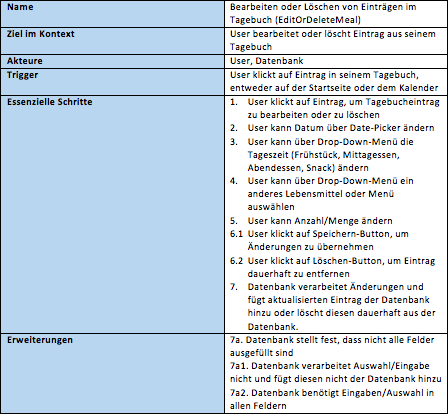
\includegraphics[scale=1]{img/usecaseeodmeal}\\
\paragraph{Datenverwaltung innerhalb der Activity}\\
Anzeige: Die Parameter werden aus dem entsprechendem Eintrag in der Kalorientagebuchtabelle geladen und im Layout angezeigt. 
Bearbeiten: Die Parameter werden in dem entsprechenden Eintrag der Kalorientagebuchtabelle angepasst.
Löschen: Der Eintrag wird aus der Datenbank komplett entfernt. 

\paragraph{Datenschnittstellen zu anderen Activity}\\
Schnittstelle zum Tagebuch (Calendar-Activity) und Startseite (Main-Activity)

\paragraph{Dokumentation des Quelltextes der Activity}\\



\subsection{Dokumentation der Navigation und des Datenaustauschs zwischen
Activities}

\subsection{Dokumentation der Activity-übergreifenden, persistenten Datenhaltung}

\subsection{Dokumentation der Activity-übergreifenden Klassen}
